In this section, we provide a basic outline of the Bayesian formalism we use to
infer the properties of the underlying GW signal, identify the most promising
events from the catalog of GW observations to base our analyses on, and discuss
the key insights they provide in constraining predictions of modified gravity
theories.

\subsection{Bayesian formalism}
If we assume that a GW signal observed in detector data $d$ is accurately
described by our waveform model \pSEOB{}, we can infer the parameters of the
model, $\bm{\lambda}$, given the hypothesis $\mathcal{H}$, using Bayes' theorem,
%
\begin{equation}
P(\bm{\lambda} \vert d, \mathcal{H}) =
\frac{p(\bm{\lambda} \vert \mathcal{H}) \, \mathcal{L}(d \vert \bm{\lambda},\mathcal{H})}{E(d \vert \mathcal{H})}\,,
\label{eq:bayes}
\end{equation}
%
where $P(\bm{\lambda} \vert d, \mathcal{H})$ is the posterior probability distribution,
$p(\bm{\lambda} \vert \mathcal{H})$ the prior,
$\mathcal{L}(d \vert \bm{\lambda},\mathcal{H})$ the likelihood, and
$E(d \vert \mathcal{H})$ the evidence.
%
The set of parameters, $\bm{\lambda}$ is a union of the GR waveform
model parameters~$\bm{\theta}$ (c.f.  Sec.~\ref{sec:review_pSEOB}), and
$\ell$,  the only non-GR parameter in this problem which, we recall, set
the characteristic length-scale in which deviations from
GR become relevant in each of the theories described in
Sec.~\ref{sec:review_theories}. Hence,
%
\begin{equation}
\bm{\lambda} = \{\ell\} \cup \{\bm{\theta}\}.
\label{eq:def_params}
\end{equation}

% As discussed in Secs.~\ref{sec:review_theories} and \ref{sec:theory_specific_qnm}, there is a single coupling
% constants in the cases of EdGB and dCS theories, but two in the cubic and
% quartic EFTofGR.
% %
% We also hold the other beyond-GR parameters, $\{\delta \omega_k^{(j)}\},$ and $\{\delta \tau_k^{(j)}\}$
% fixed to theory-specific predictions. Hence, our set of beyond--GR parameters only includes the parameter $\{\ell \}$.
% %

Assuming stationary Gaussian noise, we can write the (log) likelihood function as,
%
\begin{equation}
\ln \mathcal{L}(d \vert \bm{\lambda},\mathcal{H}) \propto
- \tfrac{1}{2}
\langle
d - h(\bm{\lambda}) \vert d - h(\bm{\lambda})
\rangle\,,
\end{equation}
%
with noise-weighted inner product $\langle \cdot | \cdot \rangle$ defined as,
%
\begin{equation}
\langle A | B \rangle =
\int_{f_{\rm low}}^{f_{\rm high}} \, \dd f \,
\frac{\tilde{A}^{\ast}(f) \tilde{B}(f) + \tilde{A}(f) \tilde{B}^{\ast}(f)}{S_{n}(f)}\,,
\end{equation}
%
where $\tilde{A}(f)$ is the Fourier transform of $A(t)$, the asterisk denotes
complex conjugation and $S_{n}(f)$ is the power spectrum density of the
detector.
%
Assuming a specific prior distribution for our parameters (discussed further in the subsequent section), we stochastically
sample over the parameter space using a Markov-Chain Monte Carlo algorithm as implemented in
\texttt{LALInferenceMCMC}~\cite{Rover:2006ni,vanderSluys:2008qx},
a package part of the \texttt{LALInference} software suite~\cite{Veitch:2014wba,lalsuite}.
%
We subsequently marginalize over the remaining parameters to obtain the
posterior probability distribution function~(PDF) on $\ell$,  i.e., $P_j(\ell \vert d_j,\mathcal{H})$,
our main parameter of interest.

For $N$ independent GW observations $\{d_j\}$, $j=1,...,N$, each characterised by a posterior probability distribution $P_j(\ell \vert d_j,\mathcal{H})$, the joint posterior can be written as:
%
\begin{equation}
P(\ell | \{d_j\}) = p(\ell) \prod_{j=1}^{N} \frac{P_j(\ell | d_j)}{p_j(\ell)}\,.
\label{eq:cumulative_dist_ell}
\end{equation}
%
where $p_j(\ell)$ are the priors used for each observation, and $p(\ell)$ is an overall prior.
%
Since we assume a uniform prior on $\ell$, the joint posterior is identically
equal to the joint likelihood.
%
In some cases, we found it necessary to work with different prior ranges across
different events, within the context of a given theory.
%
In this situation, when combining the posteriors we use chose as our overall
prior the widest one among the individual events.

\subsection{Priors}

The prior probability distribution functions on the GR parameters are assumed to be uniform over the component masses, $(m_1, m_2)$, isotropically distributed on a sphere in the sky for the source location with $p(d_L) \propto d_L^2$, and isotropic on the binary orientation, $p(\iota, \psi, \phi_0) \propto \sin\iota$. For the spins $(\chi_1, \chi_2)$, we assume a prior uniform and isotropic in the spin magnitudes and restrict ourselves to the $z$-components.
This spin-prior choice can be specified in \texttt{LALInference} using the option \texttt{alignedspin-zprior}.
%
The prior on $t_0$ is uniform and its range is informed by our detection pipelines.

Among our beyond-GR parameters, $\{\ell, \delta \omega_k^{(n)}\delta \tau_k^{(n)}\}$,
as already mentioned in the previous section, we hold $\{\delta \omega_k^{(n)}\}$
and $\{\delta \tau_k^{(n)}\}$ fixed to theory-specific predictions, and allow only $\ell$
to freely vary.
%
For such cases, we assume a prior uniform between appropriate ranges on $\ell$,
making sure that our marginalized posterior distributions on $\ell$ do not rail
over the maximum prior value on $\ell$.


\subsection{Event selection}

\begin{figure}[t]
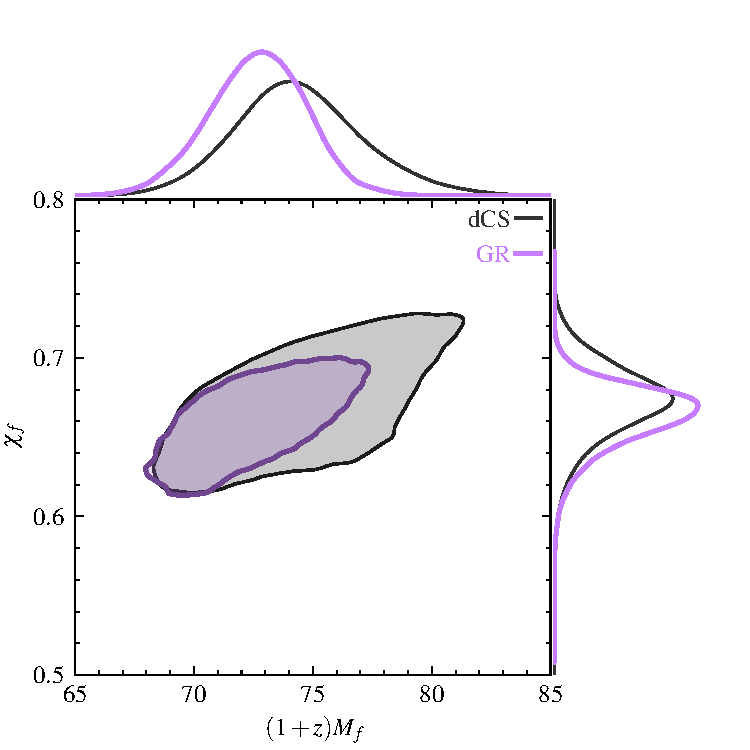
\includegraphics[width=0.9\columnwidth]{figs/tmp_GW150914_intrinsic_params_remnant.pdf}
\caption{(Color online).~Corner plot showing that the inferred final spin $\chi_f$,
detector-frame remnant mass $(1 + z) \, M_f$ for GW150915, using the same waveform model,
but without (blue contours) and with the non-GR parameters different from zero (orange contours, for
dCS gravity and $j=0$). The contours represent 90\% credible regions.
%
We see that the introduction of the non-GR parameters does not bias the
inference on the source parameters.
}
\label{fig:corner_plot}
\end{figure}

The \pSEOB{} model, as described in Sec.~\ref{sec:review_pSEOB}, is an
\emph{IMR} model which infers the properties of the underlying GW signal,
including (independently) its ringdown properties, using the Bayesian formalism
above. Naturally, the most promising candidates for our analyses are high-mass
\emph{and} loud GW observations with a significant signal-to-noise ratio (SNR)
in the post-merger part of the signal.
%
The latest LVK GW catalog~\cite{LIGOScientific:2021djp} reported 90 observed
signals not all of which are relevant for a BH ringdown analysis. In fact, in
an accompanying paper~\cite{LIGOScientific:2021sio}, the \textsc{pSEOBNRv4HM}
analysis\footnote{See, in particular, Sec.VIII A.2
in~\cite{LIGOScientific:2021sio}}, which is most similar to the \pSEOB{} model
presented in this paper, identified two events which provided the strongest
bounds on measurements of the dominant $(220)$ QNM --
GW150914~\cite{LIGOScientific:2016aoc} and
GW200129~\cite{LIGOScientific:2021djp}.
%
These two events, with a total mass of $XX \Mo$ and $XX \Mo$ respectively, are
extremely similar in their source properties. These are also two of the loudest
BBH signals observed to date with a total network SNR of XX and XX
respectively.
%
Moreover, and what is more relevant for our analysis, is their post-inspiral
(merger-ringdown) SNRs, which at XX and XX respectively (see the columns for
$\rho_{\text{post-insp}}$ in Table III of~\cite{LIGOScientific:2019fpa} and
Table IV of~\cite{LIGOScientific:2021sio}).
%
In this paper, we are going to focus on these two GW events as our probes of
the BH ringdown in modified theories of gravity.

The parameter inference in this paper follows configurations identical to the
ones used on these events for the \textsc{pSEOBNRv4HM} analysis in
Ref.~\cite{LIGOScientific:2021sio}. GW150914 was a 2-detector event (HL) while
GW200129 was 3-detector (HLV).
%
We consequently use the same strain data $h(t)$, detector
power-spectral-densities $S_n(f)$ and calibration envelopes as were used for
the analyses in Ref.~\cite{LIGOScientific:2021sio}.
%
The only difference between the sampling configurations is that we do not
sample over the fractional deviations in the $(220)$ QNM frequencies and
damping times, but instead on $\ell$ while holding $\{\delta \omega_k^{(j)}\},$
and $\{\delta \tau_k^{(j)}\}$ fixed to theory-specific predictions.
%
In the section to follow, we enumerate through the different theories and
outline the highlight results. Whenever possible, we also combine results from
multiple events to obtain the strongest possible bound on $\ell$.

% -----------------
% Corner plots here
% -----------------

As a first test ...
\hs{Move to an appendix.}

\subsection{General remarks on the interpretation of our results}
\label{sec:remarks}

There are two conditions that we must take into account before
we can confidently claim to have placed a constraint, within our model's assumptions,
with our parameter estimation study.

First, as we explained in Sec.~\ref{sec:review_theories}, all theories that we
consider must be considered as an effective field theory, meaning it should be
considered valid only below an energy scale, or equivalently, a length scale.
%
As a cut-off length scale for the validity of the EFT we use,
%
\begin{equation}
\Lambda_{\rm EFT} (\varepsilon, \mathfrak{m}) = \varepsilon \, G \mathfrak{m} / c^2 \,,
\label{eq:def_cutoff}
\end{equation}
%
where $\varepsilon$ is a dimensionless number and $\mathfrak{m}$ is the median
value of one of the mass scales involved in the problem.
%
We also momentarily restored factors of $c$ and $G$ to emphasize that $\Lambda_{\rm EFT}$ has
dimensions of length and hence can be compared to the coupling strength $\ell$.
%
In Refs.~\cite{Nair:2019iur,Perkins:2021mhb,Lyu:2022gdr}, $\varepsilon = 1/2$ was used,
but here we consider $\varepsilon \in [0, 1]$ for generality.
%
We will say that a bound has been placed on $\ell$, if most of the support of
the posterior distribution function $P(\ell)$ is in the interval
$[0, \, \Lambda_{\rm EFT}(\varepsilon, \mathfrak{m})]$.
%
In practice, this can be quantified through the cumulative distribution function
(CDF) associated with the marginalized posterior distribution $P(\ell)$, namely
%
\begin{equation}
P(\ell \leqslant \ell_{\rm max}) = \int_{-\infty}^{\,\ell_{\rm max}} P(\ell') \, \dd \ell'\,.
\label{eq:def_cdf}
\end{equation}
%
For instance, we will demand that for a bound with 90\% credibility to be meaningfully placed on $\ell$ that
%
\begin{equation}
% \textrm{CDF}(\ell) \leqslant \textrm{CDF}(T_{\rm EFT}(\varepsilon; \, \mathfrak{m})).
P(\ell \leqslant \Lambda_{\rm EFT}) \leqslant 0.9 \,,
\quad \textrm{(EFT bound)},
\label{eq:eft_bound}
\end{equation}
%
where we let $\ell_{\rm max} = \Lambda_{\rm EFT}$ in Eq.~\eqref{eq:def_cdf}, and
likewise for other credibility percentiles.

Second, as already emphasized in Ref.~\cite{Maselli:2019mjd}, the ParSpec
formalism is by construction perturbative. This means that the non-GR
deformation parameters are small, that is,
%
\begin{equation}
\gamma \, \delta \omega^{(n)} \ll 1 \,,
\,\, \textrm{and} \,\,
\gamma \, \delta \tau^{(n)} \ll 1 \,, \quad \textrm{(ParSpec bound)},
\label{eq:parspec_bound}
\end{equation}
%
for all orders $n$ in the expansion in dimensionless spin $\chi$ and where $\gamma$
is given by Eq.~\eqref{eq:def_gamma}.
%
We will also construct posterior distributions for these parameters and check if
most of their support is concentrated to a domain with values much smaller than
unity.

Another question we must consider is the following: what is the mass $\mathfrak{m}$ that we should use
in Eq.~\eqref{eq:def_cutoff}?
%
In Refs.~\cite{Nair:2019iur,Perkins:2021mhb,Lyu:2022gdr}, which attempted to
constrain dCS and shift-symmetric sGB theories with the \emph{inspiral} part of
the GW signal alone, it was natural to chose the secondary's mass $m_2$ as the most
conservative choice, since it is (by definition) the smallest mass and hence
places the lowest cut-off scale $\Lambda_{\rm EFT}$ for the validity of either of these theories as an EFT.

In our problem, the answer is not as clear. On the one hand, since we are
interested in the ringdown part of the signal, it is natural to use the
final mass $M_f$ to compute $\Lambda_{\rm EFT}$.
%
On the other hand, one may argue that the modified gravity theory under study
should be able to predict a full inspiral, merger, and ringdown of the black
hole binary before we can even make such a test, and thus the same, more conservative choice
$\gm = m_2$ should be used.
%
Here we adopt an agnostic view to this question and consider \emph{both} masses, $m_2$ and $M_f$, to
determine $\Lambda_{\rm EFT}$. We will then compare how different assumptions
yield to different interpretations of the results of our parameter estimations.


\iffalse
\subsection{Stacking posteriors}
\label{sec:stack}

If, for each event, we find that the constraints~\eqref{eq:eft_bound}
and~\eqref{eq:parspec_bound} are satisfied, we further combine the individual
posteriors distribution on $\ell$, allowing us to place a stronger bound on this parameter.
%
Let us review how do we calculate this \emph{cumulative posterior distribution} on $\ell$.

% 1. Description of data and assumption o \ell being shared
Suppose we have a data set $\{d_{i}\}$ of $N$ events which is described by
model parameters $\bm{\lambda}_{i}$, where $i$ labels each event.
%
We assume that the value of the coupling constant $\ell$, given a specific theory,
is common to all events.
%
% 2. Define joint posterior
%
The joint posterior for the parameters $\bm{\lambda}_{i}$, that describe the
data $\{d_{i}\}$, is
%
\begin{equation}
P(\ell, \{\btheta_i\} | \{d_{i}\})
= \frac{ P(\ell, \{\btheta_i\}) \, P( \{d_i\} | \ell_i, \{\btheta_i\} ) }{ P(\{d_i\}) }.
\label{eq:def_joint_posterior}
\end{equation}
%
where we separated $\ell$ from the GR waveform model parameters $\btheta$ [cf.~Eq.~\eqref{eq:def_params}].
%
% 3. Marginalisation to obtain the cumulative posterior
%
To obtain the cumulative posterior distribution on $\ell$, we marginalize
the joint posterior~\eqref{eq:def_joint_posterior} over
all parameters $\{ \btheta_i \}$, i.e.,
%
\begin{align}
P(\ell | \{d_i\}) &= \int \dd \{\btheta_i\} \, P(\ell, \{\btheta_i\} | \{d_{i}\}),
\nonumber \\
                  &= \int \dd \{\btheta_i\} \, \frac{ P(\ell, \{\btheta_i\}) \, P( \{d_i\} | \ell_i, \{\btheta_i\} ) }{ P(\{d_i\}) },
\nonumber \\
                  &= \frac{P(\ell)}{P(\{d_i\})} \int \dd \{\btheta_i\} \, P(\{\btheta_i\}) \, P( \{d_i\} | \ell, \{\btheta_i\} ),
\end{align}
%
where we have assumed that the prior on $\ell$, $P(\ell)$, is independent of
the other parameters $\{\btheta_i\}$.
%
This allow us to write $P(\ell, \{\btheta_i\} = P(\ell) P(\{\btheta_i\})$
and then move $P(\ell)$ out of the integral
%
We also moved out integral the evidence $P(\{d_i\})$, which is a normalization constant.
%
% 4. Factor the integrals in a product due to statistical independence
%
We can now factor the probabilities inside the integral, since each event is independent from another:
%
\begin{equation}
P(\ell | \{d_i\}) = \frac{P(\ell)}{P(\{d_i\})}
\prod_{i=1}^{N}
\int \dd \btheta_i \, P(\btheta_i) \, P( d_i | \ell_i, \btheta_i ).
\end{equation}
%
% 5. Final formula
We can now identify the integral as the marginalized likelihood for each individual event
%
\begin{equation}
P(\ell | \{d_i\}) = \frac{P(\ell)}{P(\{d_i\})}
\prod_{i=1}^{N} P( d_i | \ell_i ),
\end{equation}
%
which we can rewrite as
%
\begin{align}
P(\ell | \{d_i\}) &= \frac{P(\ell)}{P(\{d_i\})}
\prod_{i=1}^{N} \frac{P(d_i)}{P(\ell_i)} P(\ell_i | d_i)
\nonumber \\
&= P(\ell)
\prod_{i=1}^{N} \frac{P(\ell_i | d_i)}{P(\ell_i)}.
\label{eq:cumulative_dist_ell}
\end{align}
%
by using Bayes' theorem in the first line and cancelling the evidences in the
second line. This is our final result.

%
\hs{Abhirup, maybe move this to the subsection on priors?}
In our parameter estimation runs that we had to adjust our prior on $\ell$ depending on which event and
on which theory we examined.
%
The reasons are twofold.
%
% Describe problem 1
%
First, we found that depending on the source parameters $\btheta$,
large values of $\ell$ could result in unphysical waveforms in the frequency
band we considered. More specifically, these waveforms have a ringdown which is
considerable longer than the inspiral-merger part in the detector frequency band.
%
The fact that our sampled over these waveforms is perhaps not surprising,
because, after all, we are by construction adding corrections to the GR QNM
which \emph{increase} the damping timescale.
%
In practice, we found that these edge-cases were problematic to deal with
\texttt{LALInferenceMCMC}.
%
We overcome this problem, we reduced the prior upper-value of our prior on $\ell$.
%
This choice does not pose a problem to our parameter estimations, because these
waveforms differ grossly from the data and thus have negligible likelihood.
%
% Describe problem 2
%
However, we cannot reduce the prior on $\ell$ too much. If we do so,
to the marginalized posterior distribution on $\ell$ would rail against
the prior or, in a more extreme case, even be a uninformative, flat posterior.
%
% Summary
%
Altogether, this means that the priors $P(\ell)$ are not shared between events and
they must be taken into account when calculation the cumulative posterior function~\eqref{eq:cumulative_dist_ell}.

Finally, we use one of the approaches of Ref.~\cite{Perkins:2021mhb} to
compute the product in Eq.~\eqref{eq:cumulative_dist_ell}.
%
It method relies on first obtaining a kernel density estimator (KDE) for
the posterior distribution on $\ell$ for each individual event.
%
(See also Refs.~\cite{DelPozzo:2011pg,Cardenas-Avendano:2019zxd,Carullo:2021dui}.)
%
Next, we multiply these posteriors according to Eq.~\eqref{eq:cumulative_dist_ell}.
%
This approach based on the KDE can have difficulties in dealing with hard cut-offs in the
distribution, such as the one we impose at $\ell = 0$. We address this issue as
done in Ref.~\cite{Perkins:2021mhb}, by first doubling our number of samples as
$\{ s_i \} \cup \{ - s_i \}$, i.e., mirroring the samples across $\ell = 0$.
%
We then renormalize the associated KDE numerically in the range $\ell = [0, \infty]$.
\fi
